
\documentclass{acaces}

\begin{document}


\title{"\textit{Smart}" Manual Software Parallelisation Assistant}

\author{
Aleksandr~Maramzin\addressnum{1}\extranum{1},
Bj\"{o}rn Franke\addressnum{1}\extranum{2},
Murray Cole\addressnum{1}\extranum{2}
}

\address{1}{
Institute For Computing Systems Architecture, 
Informatics Forum, 
The University of Edinburgh, 
10 Crichton Street, 
Edinburgh, 
UK
}

\extra{1}{E-mail: s1736883@sms.ed.ac.uk}
\extra{2}{E-mail: \{bfranke,mic\}@inf.ed.ac.uk}

\pagestyle{empty}


\begin{abstract}
\quad Since automatically parallelizing compilers have failed to deliver significant performance improvements, programmers are still forced to parallelize legacy software manually for all but some niche domains. Rather than hoping for an elegant silver bullet, we acknowledge the role of a human expert in the parallelization process and develop a \textit{smart} parallelization assistant.\newline\null
\quad In its essence our assistant is yet another application of machine learning techniques to the field of optimizing compilers, which tries to predict the parallelisability property of program loops. We use Seoul National University version of NAS Parallel Benchmarks (NPB) \cite{nasa-parallel-benchmarks}, \cite{snu-npb-benchmarks} hand-annotated with OpenMP parallelisation pragmas to train our ML model. We show that the loop parallelisability classification problem can be successfully tackled with machine learning techniques (using only static code features) achieveing accuracy of around 90\% and outperforming all available baseline random predictors working at an accuracy ranging between 40\% and 70\%.\newline\null
\quad To get a real practical application of our techniques, we integrate our trained ML model into an assistant scheme, designed to mitigate the effects of ineradicable statistical errors and make them less critical. Taking application profile our assistant directs a programmer's efforts by pointing the loops, which are highly likely to be parallelisible and profitable as well. Thus, decreasing the efforts and time it takes to parallelize a program manually. As a side effect our assistant extends the capabilities of Intel C/C++ compiler in the task of parallelism discovery by increasing the amount of parallelism found in SNU NPB benchmarks from 81\% to 96\%.
\end{abstract}

\keywords{ACACES; poster session; software engineering; parallel programming; compilers; static program dependence analysis; loop iterator recognition; machine learning; programmer feedback;}

\section{Introduction}
\quad Since automatically parallelizing compilers have failed to deliver significant performance improvements, programmers are still forced to parallelize legacy software manually for all but some niche domains. Indeed, as our preliminary exploratory experiments showed the effects that Intel C/C++ Compiler (ICC) had brought with its vectorizing and parallelizing transformations to SNU NPB benchmarks ranged from no change to a significant slowdown. Rarely ICC vectorization was able to achieve a tiny speedup, but the former faded in comparison with the speedup of an expertly parallelised SNU NPB OpenMP version. Given these observations we decided to acknowledge the role of a human expert in the parallelization process and develop a \textit{smart} manual software parallelization assistant.\newline\null
\quad Our assistant is based on a ML model, trained to classify program loops as parallelisible or not. We use Seoul National University version of NAS Parallel Benchmarks (NPB) \cite{nasa-parallel-benchmarks}, \cite{snu-npb-benchmarks} hand-annotated with OpenMP parallelisation pragmas to train our ML model. We show that the loop parallelisability classification problem can be successfully tackled with machine learning techniques (using only static code features) achieveing accuracy of around 90\% and outperforming all available baseline random predictors working at an accuracy ranging between 40\% and 70\%.\newline\null
\quad The application of ML techniques to the field of parallelising compilers is not a new endeavour. As the survey of machine learning in optimising compilers \cite{mob-ml} shows there have been numerous successful application attempts. Machine learning can be used for problems ranging from selecting the best compiler flags to determining how to map parallelism to processors. Uneradicable statistical errors inherent to all ML techniques might result in the performance losses here, but do not compromise the ultimate functional correctness of the program being compiled. In this work we step into a potentially dangerous area. False positives (non-parallel loops predicted as parallelisable) can break the program. There is an already published work \cite{fried_ea:2013:icmla} studying the possibility of learning loop parallleisability property. The answer is "yes" and the work reports on a predictive performance (accuracy, recall, precision, etc.) we can achieve. But apart from studying the possibility that work does not step any further to actually find any practical utilisation of loop parallelisability predictor. Moreover, the dataset is highly unbalanced (), which sets the baseline accuracy very high. The authors use dynamic program features.\newline\null
\quad In our work we use static program features for the same loop parallelisability classification problem. We work with a more balanced dataset with richer sources of information our classification labels have been derived from. At the end we harness our trained ML model into a practical application scheme. The scheme has been designed to mitigate the effects of ineradicable statistical errors and make them less critical. Taking application profile our assistant directs a programmer's efforts by pointing the loops, which are highly likely to be parallelisible and profitable as well. Thus, decreasing the efforts and time it takes to parallelize a program manually. As a side effect our assistant extends the capabilities of Intel C/C++ compiler in the task of parallelism discovery by increasing the amount of parallelism found in SNU NPB benchmarks from 81\% to 96\%.

\section{Predicting Parallel Loops}
\label{predicting_parallel_loops}
\quad We pose a supervised ML classification problem: create a machine learning (ML) based model and train it to classify loops of Seoul National University implementation \cite{snu-npb-benchmarks} of NAS Parallel Benchmarks \cite{nasa-parallel-benchmarks} as parallelizable or not.\newline\null
\quad Our work encompasses two technical aspects we need to resolve. First, we need to find a representative set of quantifiable features, which will accurately reflect the parallelisability property of program loops. Once the feature engineering task has been done we need to select the exact ML training/testing methodology we are going to employ for our problem.\newline\null  
\quad Our features and the exact parameters of methodology (automatic feature selection methods, ML models and their hyper-parameter spaces, etc.) have been iteratively tuned and refined with the help of K-fold CV. Predictive accuracy, recall and precision scores were used as the main selection criteria. To get the most accurate and honest assessment of our ML models we kept the testing data hidden and used only the training data during all ML pipeline stages. Following subsections present the final results rather than the path towards them.
\quad We used facilities of \textit{scikit-learn} \cite{scikit-learn} Python library for all machine learning related tasks. We developed a scripting framework based on this library taking an input data (training and testing) along with a ML pipeline (methodology) configuration INI file. Configuration file allows for a flexible change in the settings of an experiment (ML model to use, its hyper-parameters, the exact automatic feature selection methods, etc.).\newline\null

\subsection{Feature Engineering}

\quad In our loop parallelisability classification problem we need to pick the right features of program loops, which are the most reflective of loop parallelisability property. In the task of coming up with a set of loop features we are guided by general program dependence analysis theory \cite{Kennedy:2001:OCM:502981}, exact types of loops present in SNU NPB benchmarks and Intel C/C++ compiler optimisation reports.\newline\null
\quad There is a range of SNU NPB loops, which escape Intel compiler parallelisation for different reasons: indirect array references, unrecognised reductions on array locations, pointers with statically unknown memory locations, etc. But all that range of different reasons is going to ultimately materialise into data and control dependencies present between loop instructions, represented as edges on the Program Dependence Graph (PDG) \cite{Ferrante:1987:PDG:24039.24041} of a loop. Figure \ref{fig:pdg} shows an example of a PDG built for a simple loop and visualised with our tool.\newline\null

\begin{figure}
\centering
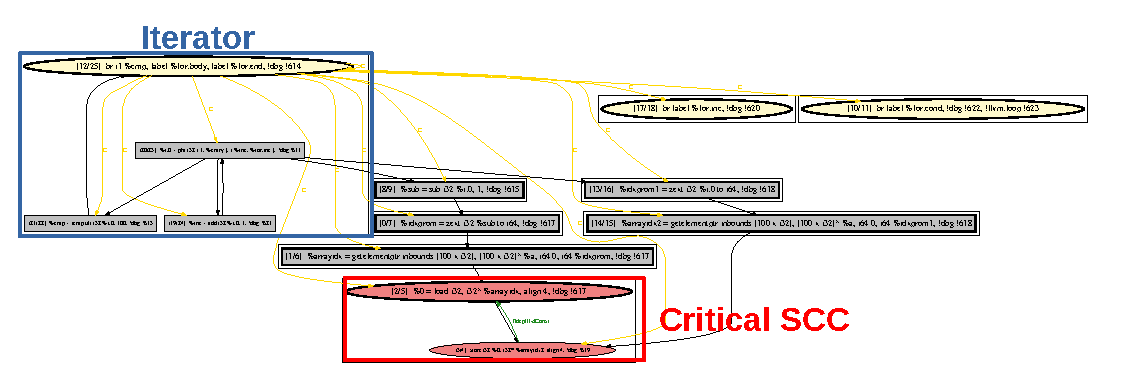
\includegraphics[width=1.0\textwidth]{pdg_example}
\caption{Program Dependence Graph of a simple loop with recognised iterator, regular and critical payload parts. Nodes are LLVM IR instructions, edges are different types of dependencies between them.}
\label{fig:pdg}
\end{figure}

\quad The PDG graph consists of LLVM IR instructions as nodes and different sorts of dependencies between them as graph edges. Dependence relation lies at the the very essence of loop parallelisation, on the other hand just counting the number of dependence edges in the PDG of a loop is not enough to make decisions about loop parallelisability. Dependence relations might exist only withing one loop iteration or span across multiple, thus preventing parallelisation.\newline\null
\quad To refine our features we use the work on generalised loop iterator recognition \cite{Manilov:2018:GPI:3178372.3179511}. Generalised iterator recognition analysis separates loop iterator from the actual payload providing us with finer loop partitions to base our features on. As work \cite{Manilov:2018:GPI:3178372.3179511} explains, loop iterator is a strongly connected component (SCC) on the PDG with no incoming dependence edges. There are SCCs in the payload as well. Usually they consist of just 1 instruction, but when we have a cross-iteration dependency they tend to grow larger and form a cycle. We call such SCCs \textit{critical}, as ones preventing parallelisation. Figure \ref{fig:pdg} highlights both the iterator and the critical SCC present in the example loop. Inner loop iterators tend to appear as critical SCCs for the outer loop as well. To separate these cases we use \textit{inner loops number} and \textit{loop depth} as separate ML features.\newline\null  
\quad The feature engineering process has been conducted iteratively and has been guided by the change in ML models predictive performance with the addition of one feature or the other. This process involved several methods. First, we tried to capture in our features the differences between PDG visualisations for parallel and non-parallel loops. Then we studied the source code of SNU NPB benchmarks along with ICC optimisation reports and tried to understand why ICC failed to parallelise some of SNU NPB loops and transfer those insights into reflective features.\newline\null
\quad We ended up with a set of 74 static loop features, which are based on the structural properties of PDG and the types of instructions constituting them. Table \ref{tab:loop_features} summarises the main groups of devised features.\newline\null
\quad Many of our features have a simple and intuitive motivations behind them. Loop proportion related features are backed up by the the fact, that bigger loops are harder to parallelise. Big iterators contain complex cross-iteration transitions (e.g linked-list update), unknown iteration numbers, etc. Critical SCCs limit loop parallelisation further. Cohesion features do not have an apparent intuition. They characterise how tightly components of loops are coupled together in terms of the number of edges between them. Loop dependencies number features count the number of edges in different loop parts as well as their types. Loop instructions nature characterise the types of loop instructions, assigning more importance to memory reads/writes, calls, branches. Uninlined funtion calls usually prevent loop parallelisation. Intensive memory work (memory read/write fraction features) complicates parallelisation as well.

\subsection{Machine Learning Methodology}

\quad The whole sequence of steps we take in order to train our model can be summarised like this: data pre  
\quad In our case we have 74 features, many of which are just slightly different variations of the same property. In order to decrease the chances of over-fitting our ML model we need to discard some features, which are redundant or irrelevant.\newline\null
\quad Our ML pipeline scripts can be configured to apply an arbitrary sequence of different feature selection methods to the provided data set. We use feature selection methods available in the scikit-learn python library. We use comparable feature selection pipelines for all the models we train. First we filter out all features with a low variance score, then we fit a decision tree based model and select all features with importance score above the threshold. Then we repeatedly run recursive feature elimination by the cross-validation (RFECV) in an attempt to improve several targets: recall, precision and accuracy scores. Table \ref{tab:best_features} illustrates the relative ranking of the 10 highest scoring features in our automatic feature selection runs.\newline\null  
\quad SNU NPB benchmarks contain a lot of uninlined function calls and it is unsurprising that the amount of call instructions in the payload of a loop ranks the highest. Despite the absence of straightforward intuition behind cohesion metrics, they tend to correlate with parallelisation labels well. Loops heavy on memory writes also significantly affect the parallelisability property.

\quad We use several machine learning algorithms available in the scikit-learn library to compare and find the best one. Among these are tree-based methods like (decision trees (DT), random forests (RFC), boosted decision trees (AdaBoost)), support vector machines (SVC) and neural network based multi-layer perceptron (MLP). Section \ref{evaluation_kfold} shows, that all these models perform comparably good with SVC and MLP being slightly better. 

\quad For any chosen parametric machine learning model we need to pick the right set of model hyper-parameters. Hyper-parameters are parameters that are not directly learnt within models. Typical examples include C, kernel and gamma for Support Vector Classifiers (SVC), exact architecture for neural network based models, etc. For any given model we use exhaustive hyper-parameter grid search and pick the node of the grid with the best cross validation score on the training set. Table presents hyper-parameter spaces we search for different models.

\quad In our work we use K-fold and modified Leave-One-Out cross-validation (LOOCV) methodologies to train and test our ML models. Detailed description of these methods can be found in the book on statistical learning \cite{James:2014:ISL:2517747}.\newline\null
\quad K-fold CV method blends all the loops from all SNU NPB benchmarks together in the single set and divides it into K equally sized splits. After that the method uses all the possible combinations of K-1 splits to train a model and test it against the one remaining split. Resulting accuracies are averaged to produce a final score. The advantage of that method in the context of our task is that it uses loops from all SNU NPB benchmarks for training and testing. When all our benchmarks differ in their, we do not miss any of them in our training process. That leads us to a better scores overall. For that reason we use that method to tune our model and report its true performance.\newline\null
\quad If we want to utilise our ML models in different practical scenarios (see section \ref{practical_applications}) we have to use separate SNU NPB benchmarks as a whole during model testing. To accomplish that we employ a modified LOOCV method to estimate the predictive performance our models can achieve against separate benchmarks in the set. Here we take all loops in every single benchmark as a testing set and train the model on all loops of 9 remaining benchmarks. The disadvantage of that method is that we exclude the whole benchmark out of the training process. If benchmark has a different nature from the ones we used to train the model, thim may come at the price of reduced accuracy.


\section{Manual Software Parallelisation Assistant}

\begin{figure}
\centering
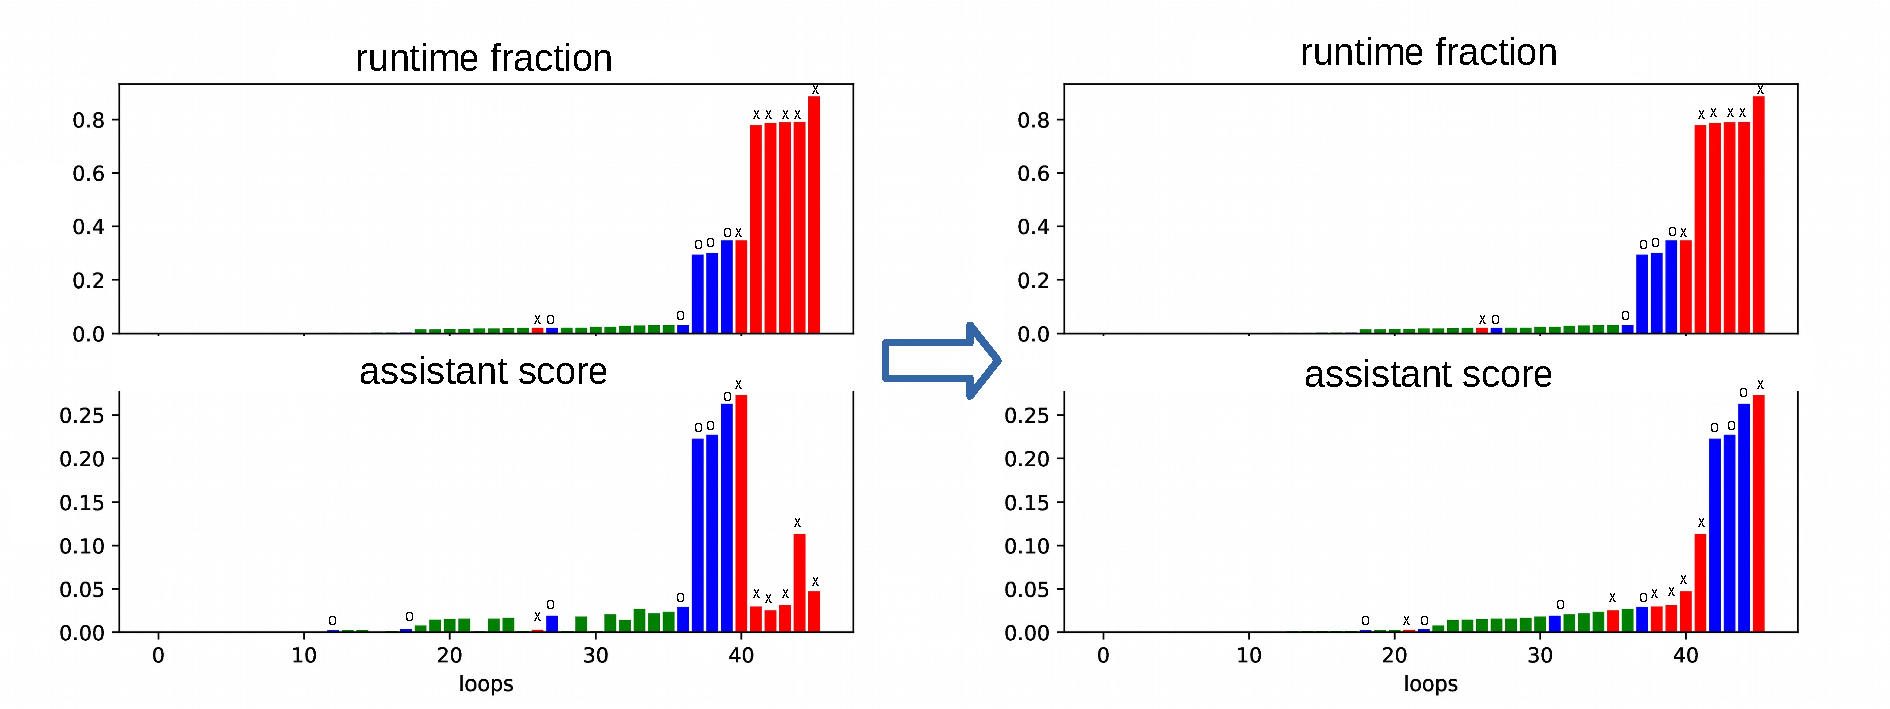
\includegraphics[width=1.0\textwidth]{ft_ranking}
\caption{Illustration of loop ranking transformation.}
\label{logo}
\end{figure}


\section{Evaluation}

\subsection{ML Model Predictive Performance}


\subsection{Assistant Scheme}

\begin{figure}
\centering
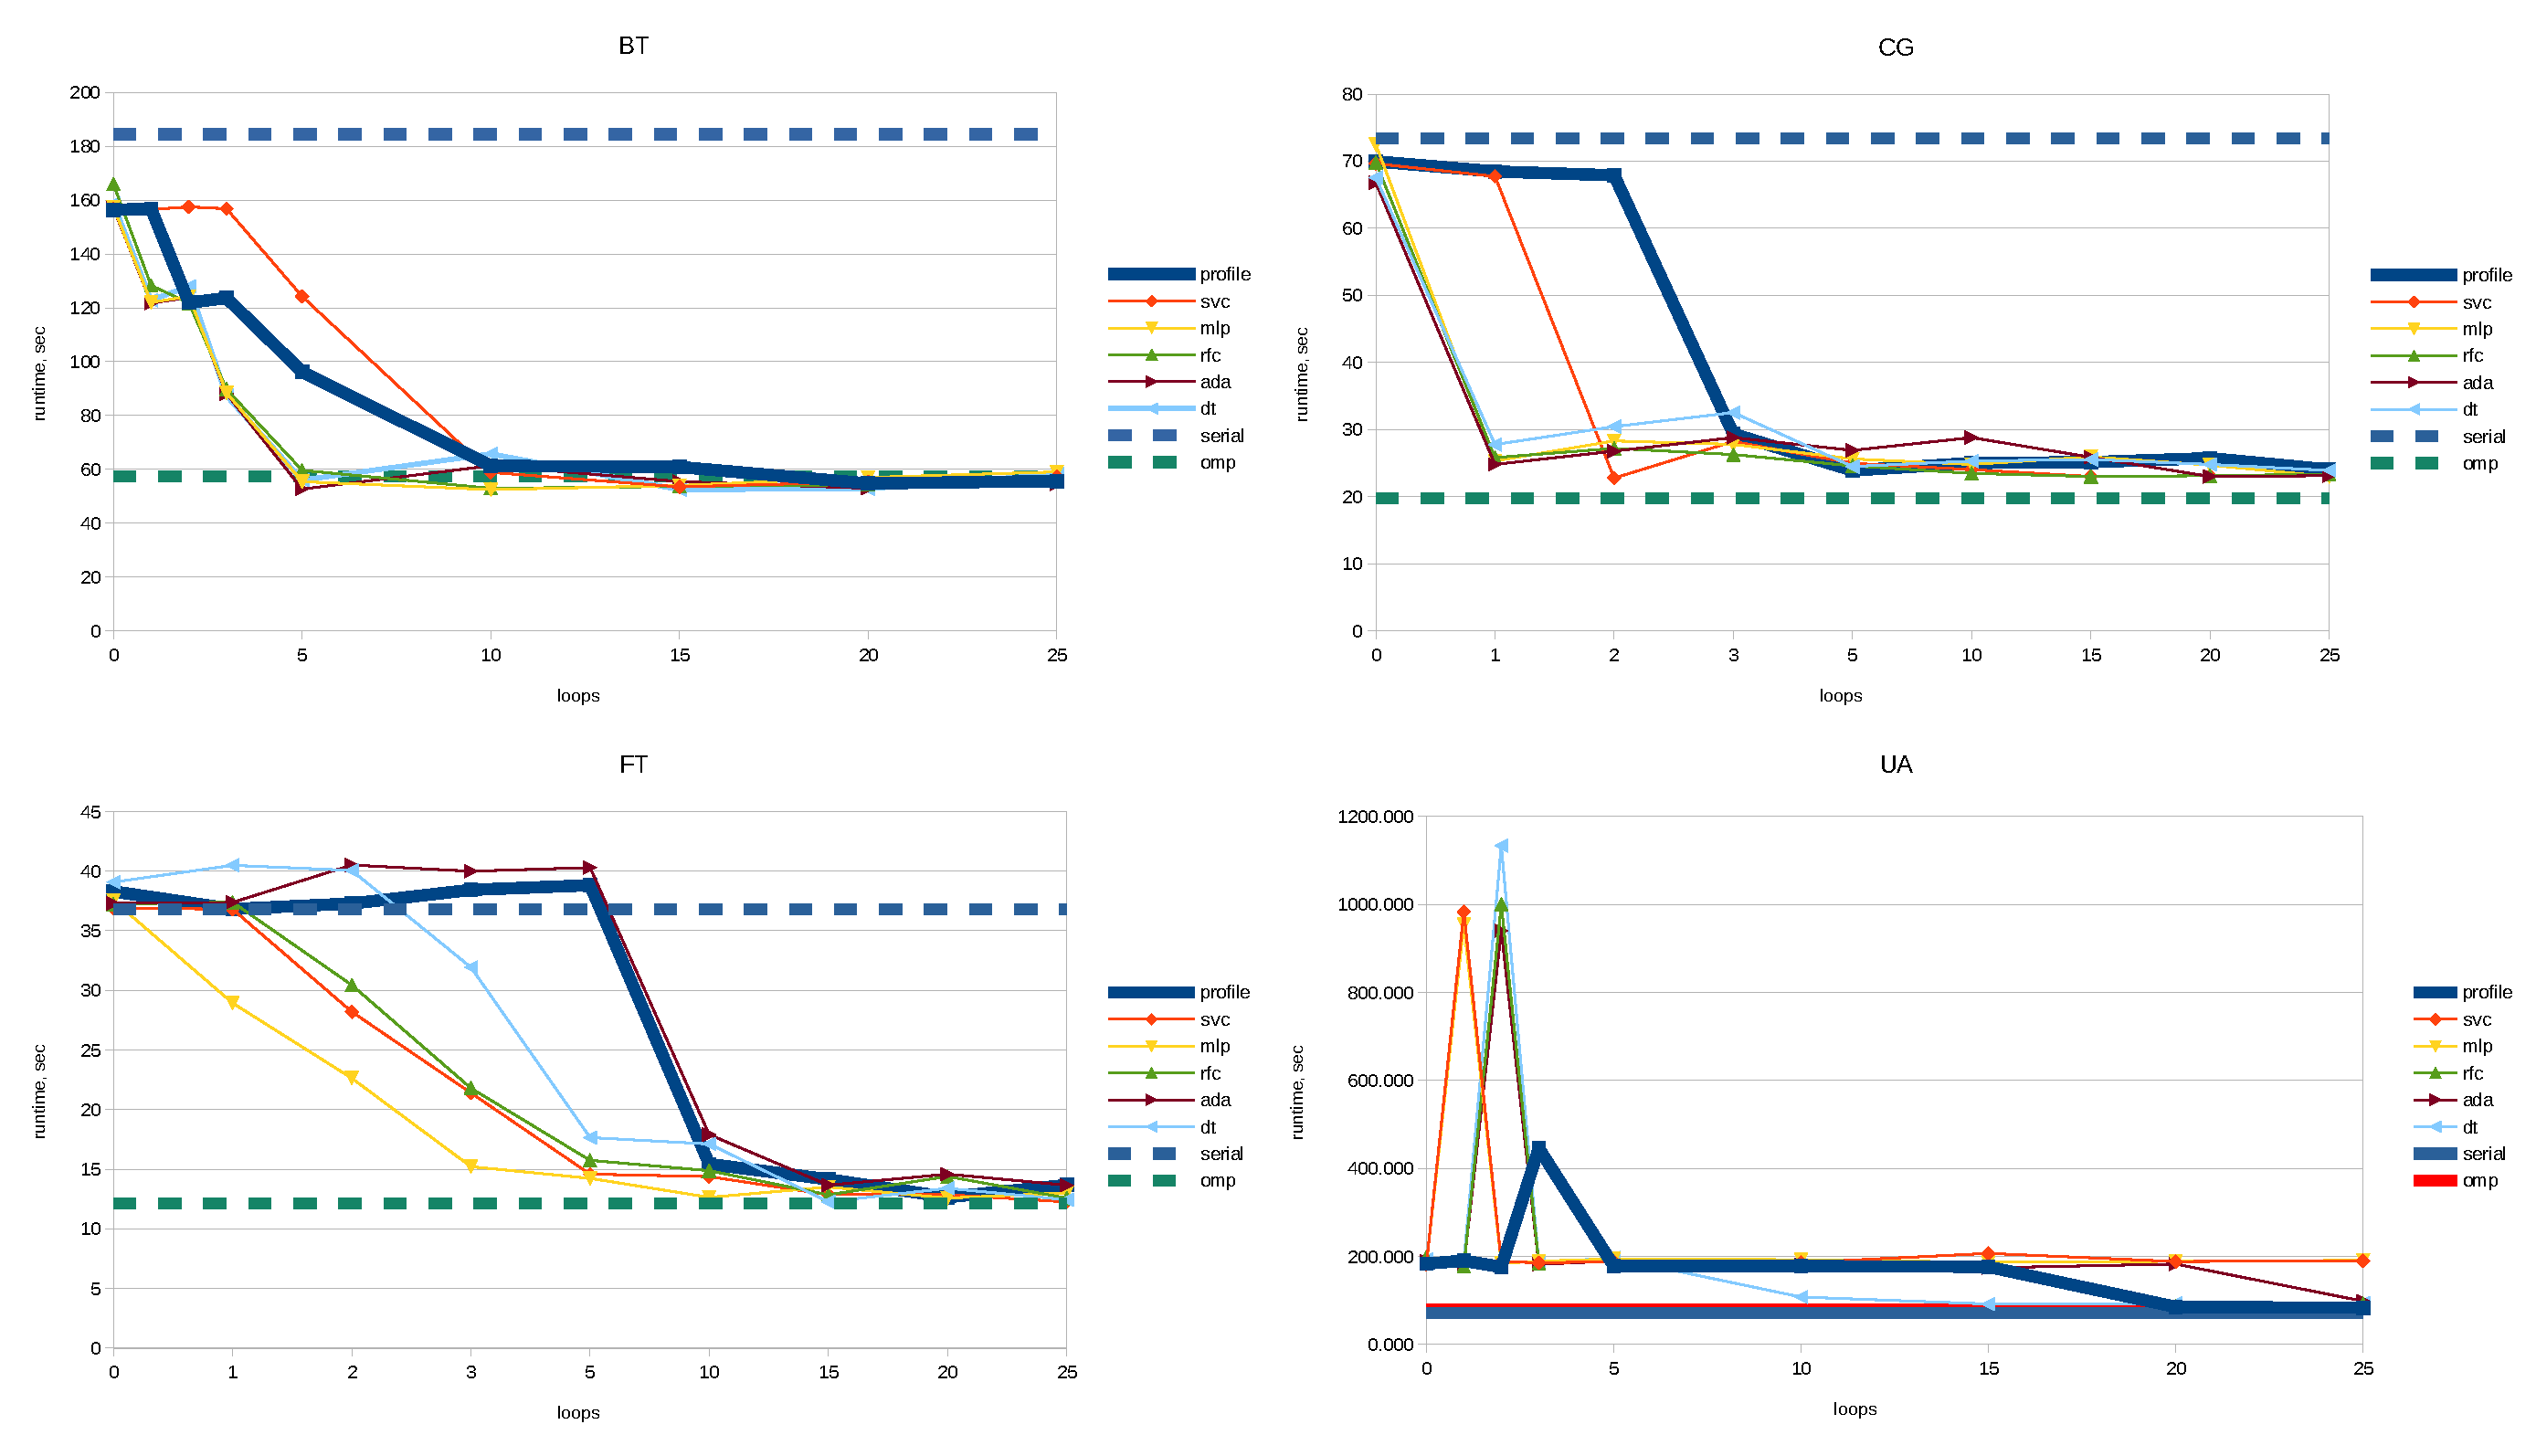
\includegraphics[width=1.0\textwidth]{parallelisation_acceleration}
\caption{Illustration of a faster convergence to the maximum achievable parallel software performance.}
\label{logo}
\end{figure}

\bibliography{guide}

\end{document}

